%\documentclass[landscape,a0b,final,a4resizeable]{a0poster}
%\documentclass[landscape,a0b,final]{a0poster}
%\documentclass[portrait,a0b,final,a4resizeable]{a0poster}
\documentclass[portrait,a0b,final]{a0poster}
%%% Option "a4resizeable" makes it possible ot resize the
%   poster by the command: psresize -pa4 poster.ps poster-a4.ps
%   For final printing, please remove option "a4resizeable" !!

\usepackage{epsfig}
\usepackage{multicol}
\usepackage{pstricks,pst-grad}
\usepackage{graphicx}% Include figure files
\usepackage{dcolumn}% Align table columns on decimal point
\usepackage{bm}% bold math
\usepackage{epsf}
\usepackage{enumitem}
\usepackage{pifont}
\usepackage{amsmath,amssymb,amsfonts}
\usepackage{xcolor}
\usepackage{tikz}
\usepackage{mathtools}


\newcommand{\bra}[1]{\left\langle #1\right|}
\newcommand{\ket}[1]{\left|#1\right\rangle}
\newcommand{\braket}[2]{\left\langle #1|#2\right\rangle}
\newcommand{\ketbrad}[1]{|#1\rangle\!\langle #1|}
\newcommand{\tr}[1]{\mathrm{tr}\left\{#1\right\}}
\newcommand{\ptr}[2]{\mathrm{tr_{#1}}\left\{#2\right\}}
\newcommand{\di}[1]{\mathrm{div}\left\{#1\right\}}
\newcommand{\la}{\left\langle}
\newcommand{\ra}{\right\rangle}
\newcommand{\pd}{\partial}
\newcommand{\de}[1]{\delta\left[#1\right]}
\newcommand{\td}{\mathrm{d}}
\newcommand{\ma}[1]{\max{\left\{#1\right\}}}
\newcommand{\mi}[1]{\min{\left\{#1\right\}}}
\newcommand{\etal}{\textit{et al. }}
\newcommand{\e}[1]{\exp{\left(#1\right)}}
\newcommand{\lo}[1]{\ln{\left(#1\right)}}
\newcommand{\id}{\mathbb{I}}
\newcommand{\com}[2]{\left[#1,\,#2\right]}
\newcommand{\acom}[2]{\left\{#1,\,#2\right\}}
\newcommand{\co}[1]{\cos{\left(#1\right)}}
\newcommand{\si}[1]{\sin{\left(#1\right)}}
\newcommand{\sh}[1]{\sinh{\left(#1\right)}}
\newcommand{\ch}[1]{\cosh{\left(#1\right)}}
\newcommand{\shi}[1]{\mathrm{shi}{\left(#1\right)}}
\newcommand{\cohi}[1]{\mathrm{chi}{\left(#1\right)}}
\newcommand{\ct}[1]{\coth{\left(#1\right)}}
\newcommand{\bla}{bla\\bla\\bla\\bla\\bla}
%\newcommand{\eqref}[1]{(\ref{#1})}
\newcommand{\PR}{Phys. Rev.}
\newcommand{\PRA}{Phys. Rev. A }
\newcommand{\PRB}{Phys. Rev. B }
\newcommand{\PRD}{Phys. Rev. D }
\newcommand{\PRE}{Phys. Rev. E }
\newcommand{\PRL}{Phys. Rev. Lett. }
\newcommand{\PRX}{Phys. Rev. X }
\newcommand{\EPL}{EPL (Europhys. Lett.) }
\newcommand{\RMP}{Rev. Mod. Phys. }
\newcommand{\NJP}{New. J. Phys. }




\newcommand{\mb}[1]{\mbox{\boldmath$#1$}}
\newcommand{\mc}[1]{\mathcal{#1}}
\newcommand{\mbb}[1]{\mathbb{#1}}
\newcommand{\mf}[1]{\mathfrak{#1}}
\newcommand{\mrm}[1]{\mathrm{#1}}
\newcommand{\clr}{\color{red}}



\newcommand{\ptl}[3]{\left( \frac{\partial {#1}}{\partial {#2}} \right)_{#3}}

\def\dbar{{\mathchar'26\mkern-12mu {\rm d}}}

\DeclareMathOperator*{\sumint}{%
\mathchoice%
  {\ooalign{$\displaystyle\sum$\cr\hidewidth$\displaystyle\int$\hidewidth\cr}}
  {\ooalign{\raisebox{.14\height}{\scalebox{.7}{$\textstyle\sum$}}\cr\hidewidth$\textstyle\int$\hidewidth\cr}}
  {\ooalign{\raisebox{.2\height}{\scalebox{.6}{$\scriptstyle\sum$}}\cr$\scriptstyle\int$\cr}}
  {\ooalign{\raisebox{.2\height}{\scalebox{.6}{$\scriptstyle\sum$}}\cr$\scriptstyle\int$\cr}}
}

\newcommand{\bull}{\ding{217}}
\newcommand{\ite}{\vspace{0.1em}\item\hspace{1em}}


%%%%%%%%%%%%%%%%%%%%%%%%%%%%%%%%%%%%%%%%%%%
% Definition of some variables and colors
%\renewcommand{\rho}{\varrho}
%\renewcommand{\phi}{\varphi}
\setlength{\columnsep}{3cm}
\setlength{\columnseprule}{1mm}
\setlength{\parindent}{0.0cm}



%%%%%%%%%%%%%%%%%%%%%%%%%%%%%%%%%%%%%%%%%%%%%%%%%%%%
%%%               Background                     %%%
%%%%%%%%%%%%%%%%%%%%%%%%%%%%%%%%%%%%%%%%%%%%%%%%%%%%
\newcommand{\background}[3]{
  \newrgbcolor{cgradbegin}{#1}
  \newrgbcolor{cgradend}{#2}
  \psframe[fillstyle=gradient,gradend=cgradend,
  gradbegin=cgradbegin,gradmidpoint=#3](0.,0.)(1.\textwidth,-1.\textheight)
}





%%%%%%%%%%%%%%%%%%%%%%%%%%%%%%%%%%%%%%%%%%%%%%%%%%%%
%%%                Poster                        %%%
%%%%%%%%%%%%%%%%%%%%%%%%%%%%%%%%%%%%%%%%%%%%%%%%%%%%

\newenvironment{poster}{
  \begin{center}
  \begin{minipage}[c]{0.98\textwidth}
}{
  \end{minipage} 
  \end{center}
}



%%%%%%%%%%%%%%%%%%%%%%%%%%%%%%%%%%%%%%%%%%%%%%%%%%%%
%%%                pcolumn                       %%%
%%%%%%%%%%%%%%%%%%%%%%%%%%%%%%%%%%%%%%%%%%%%%%%%%%%%

\newenvironment{pcolumn}[1]{
  \begin{minipage}{#1\textwidth}
  \begin{center}
}{
  \end{center}
  \end{minipage}
}



%%%%%%%%%%%%%%%%%%%%%%%%%%%%%%%%%%%%%%%%%%%%%%%%%%%%
%%%                pbox                          %%%
%%%%%%%%%%%%%%%%%%%%%%%%%%%%%%%%%%%%%%%%%%%%%%%%%%%%

\newrgbcolor{lcolor}{0. 0. 0.80}
\newrgbcolor{gcolor1}{1. 1. 1.}
\newrgbcolor{gcolor2}{.80 .80 1.}

\newcommand{\pbox}[4]{
\psshadowbox[#3]{
\begin{minipage}[t][#2][t]{#1}
#4
\end{minipage}
}}











%%%%%%%%%%%%%%%%%%%%%%%%%%%%%%%%%%%%%%%%%%%%%%%%%%%%%%%%%%%%%%%%%%%%%%
%%% Begin of Document
%%%%%%%%%%%%%%%%%%%%%%%%%%%%%%%%%%%%%%%%%%%%%%%%%%%%%%%%%%%%%%%%%%%%%%

\begin{document}

\background{0 0 0}{.99 .71 .08}{0.2}


\vspace*{1cm}


\newrgbcolor{line}{0 0 0}
\newrgbcolor{white}{.995, .995, .995}
\newrgbcolor{gray}{.97, .97, .97}
\definecolor{UMBC black}{RGB}{0 0 0}
\definecolor{UMBC gold}{RGB}{253 181 21}



\begin{poster}

%%%%%%%%%%%%%%%%%%%%%
%%% Header
%%%%%%%%%%%%%%%%%%%%%
\begin{center}
\begin{pcolumn}{0.98}

\pbox{0.97\textwidth}{0.09\textheight}{linewidth=2mm,framearc=0.3,linecolor=line,fillstyle=gradient,gradangle=0,gradbegin=white,gradend=gray,gradmidpoint=1.0,framesep=1em}{
\vspace{0.5em}
%%% Unisiegel
\begin{minipage}[c][7.5cm][c]{0.1\textwidth}
  \begin{center}
    
\includegraphics[height=7.5cm,angle=0]{UMBC-logo_small.eps}
  \end{center}
\end{minipage}
%%% Titel
\begin{minipage}[c][10cm][c]{0.78\textwidth}
  \begin{center}
    {\sc \huge Simon's algorithm in the NISQ cloud}\\[9mm]
    {\Large \textbf{Reece Robertson}, Emery Doucet, Ernest Spicer, and Sebastian Deffner\\[6mm]
    Department of Physics, University of Maryland Baltimore County, Baltimore, Maryland 21250, USA \\[1mm]
    }
  \end{center}
\end{minipage}
%%% GK-Logo
\begin{minipage}[c][7.5cm][c]{0.1\textwidth}
  \begin{center}
    
\includegraphics[height=7.5cm,angle=0]{UMBC-logo_small.eps}
  \end{center}
\end{minipage}

}
\end{pcolumn}
\end{center}


\vspace*{1cm}



%%%%%%%%%%%%%%%%%%%%%
%%% Content
%%%%%%%%%%%%%%%%%%%%%
\begin{center}
 


\begin{pcolumn}{0.495}
\pbox{0.9\textwidth}{0.09\textheight}{linewidth=2mm,framearc=0.1,linecolor=line,fillstyle=gradient,gradangle=0,gradbegin=white,gradend=white,gradmidpoint=1.0,framesep=1em}{
\vspace{1cm}\begin{center}\pbox{0.8\textwidth}{}{linewidth=2mm,framearc=0.3,linecolor=line,fillstyle=gradient,gradangle=0,gradbegin=white,gradend=gray,gradmidpoint=1.0,framesep=1em}{\begin{center}\textbf{Abstract}\end{center}}\end{center}
\vspace{1.25cm}

Simon's algorithm demonstrates genuine quantum advantage, however, it assumes access to noise-free qubits.
We use Simon's algorithm to benchmark the error rates of devices currently available in the ``quantum cloud.''
Our main result is a comparison between the platforms made available by IBM and IonQ.
This highlights the importance of understanding device architectures when transpiling quantum algorithms onto hardware.
For instance, we show that two-qubit operations between distant superconducting qubits should be avoided.

}

\vspace*{0.01\textheight}

\pbox{0.9\textwidth}{0.23\textheight}{linewidth=2mm,framearc=0.1,linecolor=line,fillstyle=gradient,gradangle=0,gradbegin=white,gradend=white,gradmidpoint=1.0,framesep=1em}{
\vspace{1cm}\begin{center}\pbox{0.8\textwidth}{}{linewidth=2mm,framearc=0.3,linecolor=line,fillstyle=gradient,gradangle=0,gradbegin=white,gradend=gray,gradmidpoint=1.0,framesep=1em}{\begin{center}\textbf{Background}\end{center}}\end{center}\vspace{1.25cm}

\textbf{Simon's problem:}
\begin{itemize}
  \item Input: a black-box oracle function $U_f$ which operates on bitstrings of size $n$.
  \begin{itemize}
    \item $U_f$ is two-to-one with a ``secret string'' $s$ that relates input pairs.
  \end{itemize}
  \item Objective: Determine $s$ where the only allowable action is to make queries to $U_f$.
  \item Classical runtime is exponential in $n$. Quantum runtime is linear in $n$.
\end{itemize}

\begin{center}
  
\includegraphics[height=4.5cm,angle=0]{genericAlgorithm.png}
\end{center}

\textbf{Simon's Algorithm:}~\cite{ref1}
\begin{enumerate}
  \item Initialize two quantum registers of size $n$ in the $|0\rangle$ state.
  \item Apply two Hadamard transformations and $U_f$ to the registers as depicted above.
  \begin{itemize}
    \item This creates a superposition in the first register over all size $n$ bitstrings that are orthogonal to $s$.
  \end{itemize}
  \item Measure the registers to obtain a single size $n$ bitstring that is orthogonal to $s$.
\end{enumerate}
By iterating steps 1-3 to form a set of $n-1$ linearly independent bitstrings we can solve for $s$.

}

\vspace*{0.01\textheight}

\pbox{0.9\textwidth}{0.45\textheight}{linewidth=2mm,framearc=0.1,linecolor=line,fillstyle=gradient,gradangle=0,gradbegin=white,gradend=white,gradmidpoint=1.0,framesep=1em}{
\vspace{1cm}\begin{center}\pbox{0.8\textwidth}{}{linewidth=2mm,framearc=0.3,linecolor=line,fillstyle=gradient,gradangle=0,gradbegin=white,gradend=gray,gradmidpoint=1.0,framesep=1em}{\begin{center}\textbf{The Quantum Cloud}\end{center}}\end{center}\vspace{1.25cm}

Several large corporations as well as smaller start-up companies have made their NISQ devices available for cloud access.
For our study, we had access to IBM's superconducting platform and IonQ's trapped ion devices.

\textbf{Superconducting qubits -- IBM:}
\begin{itemize}
  \item Quantum processors made of superconducting transmon qubits.
  \item Physically located in dilution refrigerators at the Thomas J. Watson Research Center.
  \item Largest existing processor has 1,121 qubits.
  \item Chip topology limited to pairwise connections between qubits.
  \item We used the 127-qubit Brisbane, Osaka, and Kyoto (all instances of the Eagle chip design below).
  \item Noisy simulator models provided by IBM for these devices.
\end{itemize}

\begin{center}
  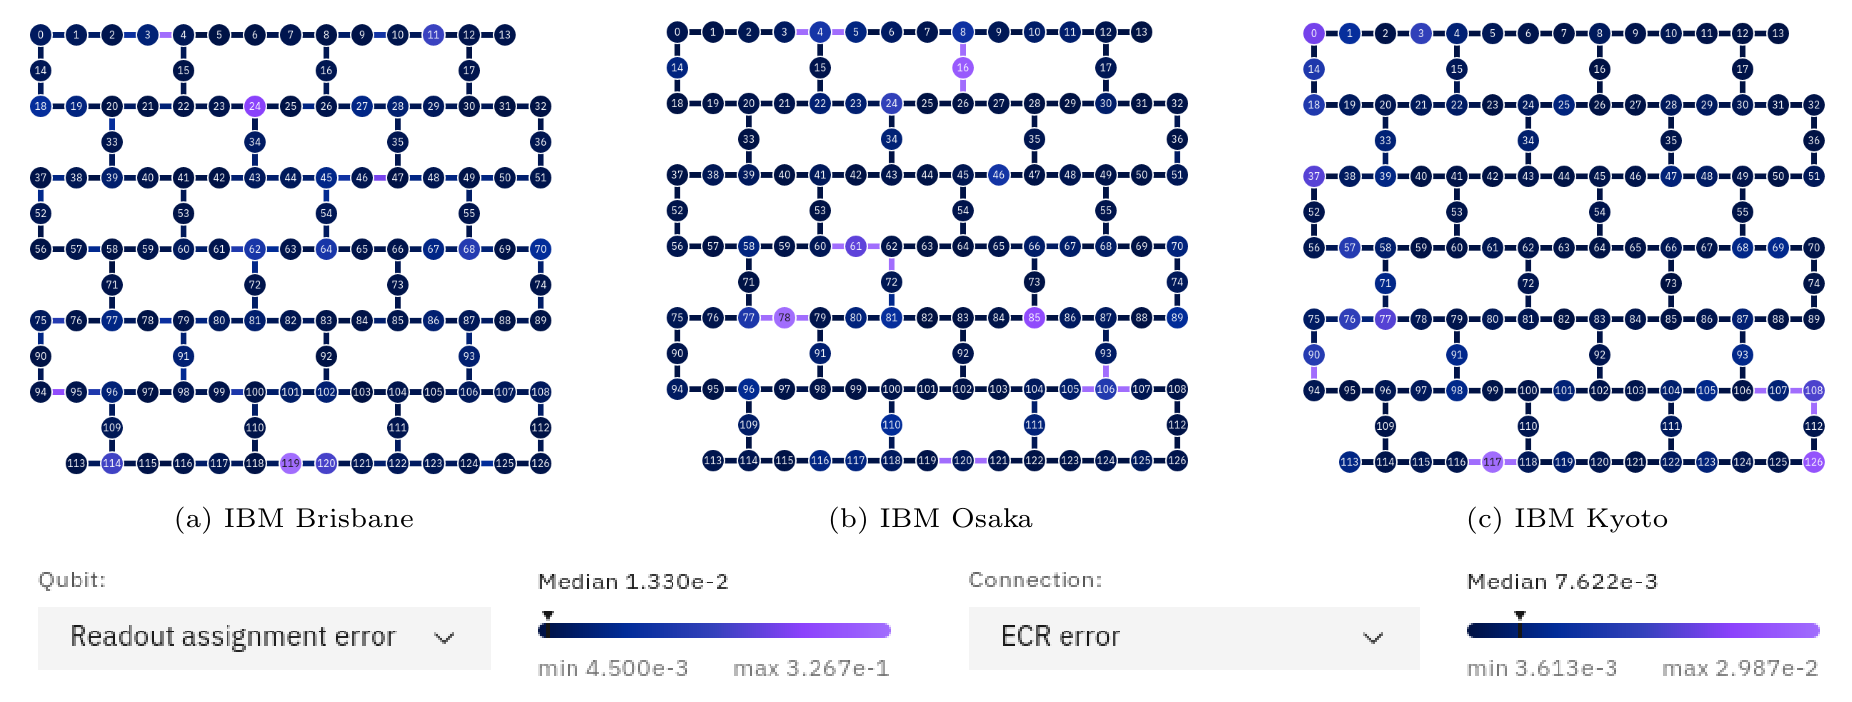
\includegraphics[height=12cm,angle=0]{ibmDevices.png}
\end{center}

\textbf{Ion traps -- IonQ:}
\begin{itemize}
  \item Quantum processors made of trapped ions.
  \item Physically located here in College Park.
  \item Largest existing processor has 36 qubits.
  \item Chip topology allows for all-to-all qubit connectivity.
  \item We used the 11-qubit Harmony, 25-qubit Aria, and 36-qubit Forte.
  \item Noisy simulator models provided by IonQ for Harmony and Aria.
\end{itemize}

\begin{center}
  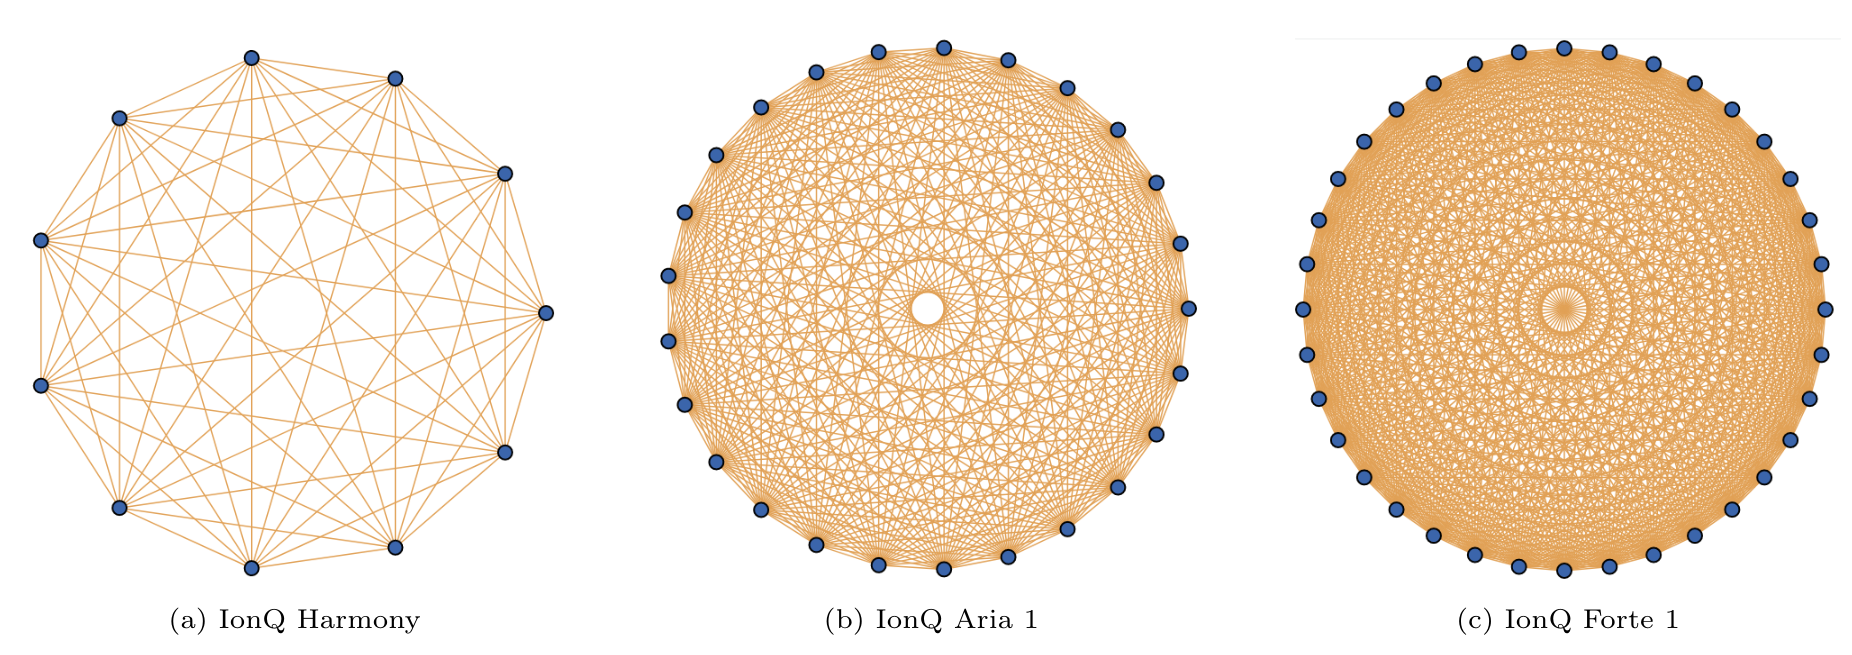
\includegraphics[height=12cm,angle=0]{ionqDevices.png}
\end{center}

}

\end{pcolumn}
\begin{pcolumn}{0.495}
\pbox{0.9\textwidth}{0.54\textheight}{linewidth=2mm,framearc=0.1,linecolor=line,fillstyle=gradient,gradangle=0,gradbegin=white,gradend=white,gradmidpoint=1.0,framesep=1em}{

\vspace{1cm}\begin{center}\pbox{0.8\textwidth}{}{linewidth=2mm,framearc=0.3,linecolor=line,fillstyle=gradient,gradangle=0,gradbegin=white,gradend=gray,gradmidpoint=1.0,framesep=1em}{\begin{center}\textbf{Methods \& Results}\end{center}}\end{center}\vspace{1.25cm}

\textbf{Methods:}

Our objective was to determine the frequency with which Simon's algorithm failed on NISQ technology.
To this end, we ran Simon's algorithm on the devices and simulator listed previously using the following process:
\begin{enumerate}
  \item We initialized a variable $n$ to iterate over the values 2—12.
  \item For each $n$, we defined a two-to-one function using the string of $n$ 1s as the secret string $s$.
  \begin{itemize}
    \item This represents the most complex oracle in terms of the number of two-qubit gates required.
  \end{itemize}
  \item We prepared an implementation of Simon's algorithm to classify this function.
  \item We repeated the implementation for 8192 shots.
  \item We counted the fraction of shots that produced a final result \textit{not} orthogonal to $s$---the \textit{algorithmic error}.
  \begin{itemize}
    \item These shots indicate presence of hardware noise which resulted in a failure of the implementation.
  \end{itemize}
  \item We averaged the algorithmic error of each device over many repetitions of steps 1-5, and plotted the results.
\end{enumerate}

\textbf{IBM Results:}
\begin{itemize}
  \item IBM simulators predict a roughly linear scaling in algorithmic error as a function of $n$.
  \item IBM devices experience a nonlinear jump in algorithmic error at $2n=8$ (or $2n=10$ for Kyoto).
  \begin{itemize}
    \item This increase in error on hardware coincides with the addition of swap gates into the algorithm.
    \item These swap operations may introduce correlated errors not captured in the simulators' noise model.
  \end{itemize}
  \item The observed 50\% algorithmic error for $2n\geq12$ demonstrates a failure of the algorithm.
\end{itemize}

\begin{center}
  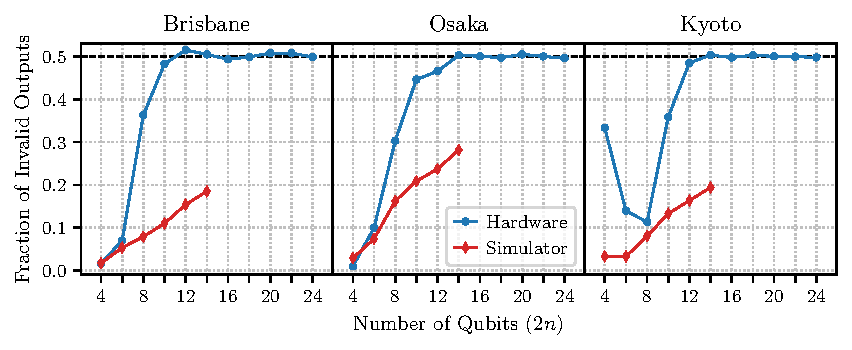
\includegraphics[height=12cm,angle=0]{IBMComparisonTest.pdf}
\end{center}

\textbf{IonQ Results:}
\begin{itemize}
  \item IonQ simulators predict a roughly linear scaling in algorithmic error as a function of $n$.
  \item IonQ devices demonstrate a roughly linear scaling in algorithmic error as a function of $n$.
  \item On Aria, there is a roughly constant factor of 2 difference between the simulator and hardware results.
  \item The observed 30\% algorithmic error for $2n\geq24$ will likely nullify quantum advantage.
\end{itemize}

\begin{center}
  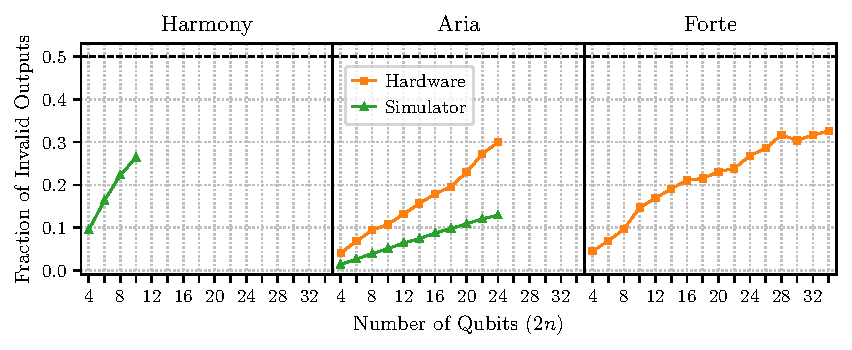
\includegraphics[height=12cm,angle=0]{IonQComparisonTest.pdf}
\end{center}

In sum, we find that the algorithmic error of Simon's algorithm on NISQ devices scales at least linearly, and all devices show irrecoverable error for intermediate-scale problems ($2n=24$).

}

\vspace*{0.01\textheight}


\pbox{0.9\textwidth}{0.20\textheight}{linewidth=2mm,framearc=0.1,linecolor=line,fillstyle=gradient,gradangle=0,gradbegin=white,gradend=white,gradmidpoint=1.0,framesep=1em}{

\vspace{1cm}\begin{center}\pbox{0.8\textwidth}{}{linewidth=2mm,framearc=0.3,linecolor=line,fillstyle=gradient,gradangle=0,gradbegin=white,gradend=gray,gradmidpoint=1.0,framesep=1em}{\begin{center}\textbf{Physical Parameters of the NISQ Devices}\end{center}}\end{center}\vspace{1.25cm}

\begin{center}
  \begin{tabular}{|c|c|c|c|c|c|c|}
    \hline
    Parameter & Brisbane & Osaka & Kyoto & Forte & Aria 1 & Harmony \\
    \hline
    \hline
    Manufacturer & IBM & IBM & IBM & IonQ & IonQ & IonQ \\
    \hline
    T1 Time & 213.12 $\mu$s & 297.17 $\mu$s & 215.43 $\mu$s & 100 s & 100 s & 10000 s \\
    \hline
    T2 Time & 145.97 $\mu$s & 127.23 $\mu$s & 109.44 $\mu$s & 1 s & 1 s & 0.2 s \\
    \hline
    2-Qubit Gate Speed & 660 ns & 660 ns & 660 ns & 970 $\mu$s & 600 $\mu$s & 200 $\mu$s \\
    \hline
    1-Qubit Gate Error (\%) & 0.03 & 0.03 & 0.03 & 0.09 & 0.06 & 0.67 \\
    \hline
    2-Qubit Gate Error (\%) & 0.74 & 0.93 & 0.92 & 0.74 & 8.57 & 3.07 \\
    \hline
    Average Readout Error (\%) & 1.32 & 2.18 & 1.48 & 0.5 & 0.52 & 0.42 \\
    \hline
    Topology & Eagle r3 & Eagle r3 & Eagle r3 & all-to-all & all-to-all & all-to-all \\
    \hline
  \end{tabular}
\end{center}

\textbf{Notes:}
\begin{itemize}
  \item IBM reports median values; IonQ reports average values.
  \item IBM native gate set: ECR, ID, RZ, SX, and X.
  \item IonQ native gate set: MS, GPI, and GPI2 (Forte includes ZZ).
\end{itemize}

}

\vspace*{0.01\textheight}

\pbox{0.9\textwidth}{0.03\textheight}{linewidth=2mm,framearc=0.1,linecolor=line,fillstyle=gradient,gradangle=0,gradbegin=white,gradend=white,gradmidpoint=1.0,framesep=1em}{


%%% References
\begin{thebibliography}{80}

\bibitem{ref1} D. R. Simon, On the power of quantum computation, SIAM Journal on Computing 26 (5) (1997) 1474--1483. arXiv:
https://doi.org/10.1137/S0097539796298637, doi:10.1137/S0097539796298637.

\end{thebibliography}
}

\end{pcolumn}

\end{center}

\end{poster}

\end{document}

\bib